% -*- latex -*-
%%%%%%%%%%%%%%%%%%%%%%%%%%%%%%%%%%%%%%%%%%%%%%%%%%%%%%%%%%%%%%%%
%%%%%%%%%%%%%%%%%%%%%%%%%%%%%%%%%%%%%%%%%%%%%%%%%%%%%%%%%%%%%%%%
%%%%
%%%% This text file is part of the source of 
%%%% `Parallel Programming in MPI and OpenMP'
%%%% by Victor Eijkhout, copyright 2012-2021
%%%%
%%%% mpi-io.tex : MPI/O
%%%%
%%%%%%%%%%%%%%%%%%%%%%%%%%%%%%%%%%%%%%%%%%%%%%%%%%%%%%%%%%%%%%%%
%%%%%%%%%%%%%%%%%%%%%%%%%%%%%%%%%%%%%%%%%%%%%%%%%%%%%%%%%%%%%%%%

\index{MPI/O|(}

This chapter discusses the I/O support of MPI, which is intended
to alleviate the problems inherent in parallel file access.
Let us first explore the issues.
This story partly depends on what sort of parallel
computer are you running on.
Here are some of the hardware scenarios you may encounter:

\begin{itemize}
\item On networks of workstations each node will have a separate
  drive with its own file system.
\item On many clusters there will be a
  \emph{shared file system}\index{file system!shared}
  that acts as if every process can access every file.
\item Cluster nodes may or may not have a private file system.
\end{itemize}

Based on this, the following strategies are possible, even before
we start talking about MPI I/O.

\begin{itemize}
\item One process can collect all data with \indexmpishow{MPI_Gather}
  and write it out. There are at least three things wrong with this:
  it uses network bandwidth for the gather, it may require a large
  amount of memory on the root process, and centralized writing
  is a bottleneck.
\item Absent a shared file system, writing can be parallelized by letting
  every process create a unique file and merge these after the run.
  This makes the I/O symmetric, but collecting all the files is a bottleneck.
\item Even with a with a shared file system this approach is possible,
  but it can put a lot of strain
  on the file system, and the post-processing can be a significant task.
\item Using a shared file system,
  there is nothing against every process opening the same existing file
  for reading, and using an individual file pointer to get its unique
  data.
\item \ldots~but having every process open the same file for output is
  probably not a good idea. For instance, if two processes try to write
  at the end of the file, you may need to synchronize them, and synchronize
  the file system flushes.
\end{itemize}

For these reasons, MPI has a number of routines that make it possible
to read and write a single file from a large number of processes,
giving each process its own well-defined location where to access the data.
These locations can use MPI
\indextermsub{derived}{datatype}s for both the source data (that is, in memory)
and target data (that is, on disk).
Thus, in one call that is collective on a communicator
each process can address data that is not contiguous in memory,
and place it in locations that are not contiguous on disc.

There are dedicated libraries for file I/O, such as \indexterm{hdf5},
\indexterm{netcdf}, or \indexterm{silo}. However, these often add
header information to a file that may not be understandable to
post-processing applications. With MPI I/O you are in complete control
of what goes to the file. (A~useful tool for viewing your file is the
unix utility~\indextermtt{od}.)

\begin{taccnote}
  Each node has a private \verb+/tmp+ file system
  (typically flash storage), to which
  you can write files. Considerations:
  \begin{itemize}
  \item Since these drives are separate from the shared file system,
    you don't have to worry about stress on the file servers.
  \item These temporary file systems are wiped after your job finishes,
    so you have to do the post-processing in your job script.
  \item The capacity of these local drives are fairly limited;
    see the userguide for exact numbers.
  \end{itemize}
\end{taccnote}

\Level 0 {File handling}

MPI has a datatype for files: \indexmpidef{MPI_File}.
This acts a little like a traditional file handle,
in that there are open, close, read/write, and seek operations on it.
However, unlike traditional file handling,
which in parallel would mean having one handle per process,
this handle is collective: MPI processes
act as if they share one file handle.

You open a file with
%
\indexmpiref{MPI_File_open}.
%
This routine is collective, even if only certain processes will access
the file with a read or write call.
Similarly, \indexmpidef{MPI_File_close} is collective.

\begin{pythonnote}{File open is class method}
  Note the slightly unusual syntax for opening a file:
\begin{lstlisting}
mpifile = MPI.File.Open(comm,filename,mode)
\end{lstlisting}
  Even though the file is
  opened on a communicator, it is a class method for the \n{MPI.File}
  class, rather than for the communicator object. The latter is passed
  in as an argument.
\end{pythonnote}

File access modes:
\begin{itemize}
\item  \indexmpidef{MPI_MODE_RDONLY}: read only,
\item  \indexmpidef{MPI_MODE_RDWR}: reading and writing,
\item  \indexmpidef{MPI_MODE_WRONLY}: write only,
\item  \indexmpidef{MPI_MODE_CREATE}: create the file if it does not exist,
\item  \indexmpidef{MPI_MODE_EXCL}: error if creating file that already exists,
\item  \indexmpidef{MPI_MODE_DELETE_ON_CLOSE}: delete file on close,
\item  \indexmpidef{MPI_MODE_UNIQUE_OPEN}: file will not be concurrently opened
  elsewhere,
\item  \indexmpidef{MPI_MODE_SEQUENTIAL}: file will only be accessed sequentially,
\item  \indexmpidef{MPI_MODE_APPEND}: set initial position of all file pointers to end
  of file.
\end{itemize}
These modes can be added or bitwise-or'ed.

As a small illustration:
%%
\csnippetwithoutput{mpifilebasic}{examples/mpi/c}{write}

You can delete a file with \indexmpidef{MPI_File_delete}.

Buffers can be flushed with \indexmpidef{MPI_File_sync}, which is a collective call.

\Level 0 {File reading and writing}

The basic file operations, in between the open and close calls, are
the POSIX-like, noncollective, calls
\begin{itemize}
\item \indexmpiref{MPI_File_seek}. The \lstinline{whence} parameter can be:
  \begin{itemize}
  \item \indexmpidef{MPI_SEEK_SET} The pointer is set to offset.
  \item \indexmpidef{MPI_SEEK_CUR} The pointer is set to the current
    pointer position plus offset.
  \item \indexmpidef{MPI_SEEK_END} The pointer is set to the end of
    the file plus offset.
  \end{itemize}
\item \indexmpiref{MPI_File_write}. This routine writes the specified data
  in the locations specified with the current file view. 
  The number of items written is returned in the \indexmpishow{MPI_Status} argument;
  all other fields of this argument are undefined.
  It can not be used if the file
  was opened with \indexmpishow{MPI_MODE_SEQUENTIAL}.
\item If all processes execute a write at the same logical time, it is
  better to use the collective call
  \indexmpidef{MPI_File_write_all}.
\item \indexmpiref{MPI_File_read} This routine attempts to read the specified data
  from the locations specified in the current file view. 
  The number of items read is returned in the \indexmpishow{MPI_Status} argument;
  all other fields of this argument are undefined.
  It can not be used if the file
  was opened with \indexmpishow{MPI_MODE_SEQUENTIAL}.
\item If all processes execute a read at the same logical time, it is
  better to use the collective call
  \indexmpiref{MPI_File_read_all}.
\end{itemize}

For thread safety it is good to combine seek and read/write operations:
\begin{itemize}
\item \indexmpidef{MPI_File_read_at}: combine read and seek.
  The collective variant is \indexmpidef{MPI_File_read_at_all}.
\item \indexmpishow{MPI_File_write_at}: combine write and seek.
  The collective variant is \indexmpidef{MPI_File_write_at_all};
  section~\ref{sec:mpi-filepoint}.
\end{itemize}

Writing to and reading from a parallel file is rather similar to
sending a receiving:
\begin{itemize}
\item The process uses an elementary data type or a derived datatype
  to describe what elements in an array go to file, or are read from
  file.
\item In the simplest case, your read or write that data to the file using an
  offset, or first having done a seek operation.
\item But you can also set a `file view' to describe explicitly what
  elements in the file will be involved.
\end{itemize}

\Level 1 {Nonblocking read/write}

Just like there are blocking and nonblocking sends, there are also
nonblocking writes and reads:
\indexmpiref{MPI_File_iwrite},
\indexmpidef{MPI_File_iread} 
operations,
and their collective versions
\indexmpidef{MPI_File_iwrite_all},
\indexmpidef{MPI_File_iread_all}.

Also 
\indexmpidef{MPI_File_iwrite_at},
\indexmpidef{MPI_File_iwrite_at_all},
\indexmpidef{MPI_File_iread_at}.,
\indexmpidef{MPI_File_iread_at_all}.

These routines output an \indexmpishow{MPI_Request} object,
which can then be tested with
\indexmpishow{MPI_Wait} or \indexmpishow{MPI_Test}.

Nonblocking collective I/O functions
much like other nonblocking collectives
(section~\ref{sec:mpi3collect}):
the request is satisfied if all processes finish the collective.

There are also \indextermsub{split}{collective}s
that function like nonblocking collective I/O, but with the request/wait mechanism:
\indexmpidef{MPI_File_write_all_begin}~/
\indexmpidef{MPI_File_write_all_end}
(and similarly
\indexmpidef{MPI_File_read_all_begin}~/
\indexmpidef{MPI_File_read_all_end})
where the second routine blocks until the collective write/read
has been concluded.

Also \indexmpishow{MPI_File_iread_shared}, \indexmpishow{MPI_File_iwrite_shared}.

\Level 1 {Individual file pointers, contiguous writes}
\label{sec:mpi-filepoint}

After the collective open call, each process holds an
\emph{individual file pointer}\index{file!pointer!individual}
that it can individually position somewhere in the shared file.
Let's explore this modality.

The simplest way of writing a data to file is much like a send call:
a~buffer is specified with the usual count/datatype specification,
and a target location in the file is given.
The routine \indexmpiref{MPI_File_write_at} gives this location
in absolute terms with a parameter of type \indexmpidef{MPI_Offset},
which counts bytes.

\begin{figure}[ht]
  \label{fig:write-at}
  \caption{Writing at an offset}
  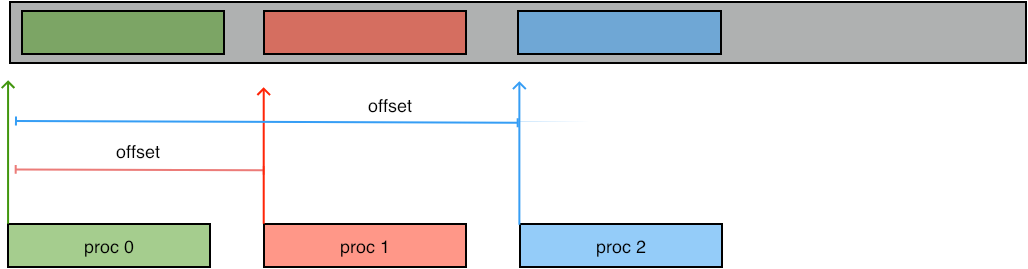
\includegraphics[scale=.4]{write-at-offset}
\end{figure}

\begin{exercise}
  \label{ex:blockwrite}
  Create a buffer of length \n{nwords=3} on each process, and write
  these buffers as a sequence to one file with \indexmpishow{MPI_File_write_at}.
  \skeleton{blockwrite}
\end{exercise}

Instead of giving the position in the file explicitly, you can also
use a \indexmpishow{MPI_File_seek} call to position the file pointer,
and write with \indexmpishow{MPI_File_write} at the pointer location.
The write call itself also 
\emph{advances the file pointer}\index{file!pointer!advance by write}
so separate calls for writing contiguous elements 
need no seek calls with \indexmpishow{MPI_SEEK_CUR}.

\begin{exercise}
  \label{ex:blockadvance}
  Rewrite the code of exercise~\ref{ex:blockwrite} to
  use a loop where each iteration
  writes only one item to file.
  Note that no explicit advance of the file pointer is needed.
\end{exercise}

\begin{exercise}
  \label{ex:blockseek}
  Construct a file with the consecutive integers $0,\ldots,WP$ where
  $W$~some integer, and $P$~the number of processes. Each process~$p$
  writes the numbers $p,p+W,p+2W,\ldots$. Use a loop where each iteration
  \begin{enumerate}
  \item writes a single number with \lstinline{MPI_File_write}, and
  \item advanced the file pointer with \indexmpishow{MPI_File_seek}
    with a \lstinline{whence} parameter of
    \indexmpishow{MPI_SEEK_CUR}.
  \end{enumerate}
\end{exercise}

\Level 1 {File views}

The previous mode of writing is enough for writing simple contiguous blocks in the file.
However,
you can also access noncontiguous areas in the file. For this you use
%
\indexmpiref{MPI_File_set_view}.
%
This call is collective, even if not all processes access the file.
\begin{itemize}
\item The \n{disp} displacement parameters is measured in bytes. It
  can differ between processes. On sequential files such as tapes or
  network streams it does not make sense to set a displacement; for
  those the \indexmpidef{MPI_DISPLACEMENT_CURRENT} value can be
  used.
\item The \n{etype} describes the data type of the file, it needs to
  be the same on all processes.
\item The \n{filetype} describes how this process sees the file, so it
  can differ between processes.
\item The \n{datarep} string can have the following values:
  \begin{itemize}
  \item \n{native}: data on disk is represented in exactly the same
    format as in memory;
  \item \n{internal}: data on disk is represented in whatever internal
    format is used by the MPI implementation;
  \item \n{external}: data on disk is represented using XDR portable
    data formats.
  \end{itemize}
\item The \n{info} parameter is an \indexmpishow{MPI_Info} object,
  or \indexmpishow{MPI_INFO_NULL}.
  See section~\ref{sec:mpi-info-file} for more on file info.
  (See \indextermdef{T3PIO}~\cite{t3pio-git} for a tool that 
  assists in setting this object.)
\end{itemize}

\cverbatimsnippet{mpiviewnative}

\begin{figure}[ht]
  \label{fig:write-view}
  \caption{Writing at a view}
  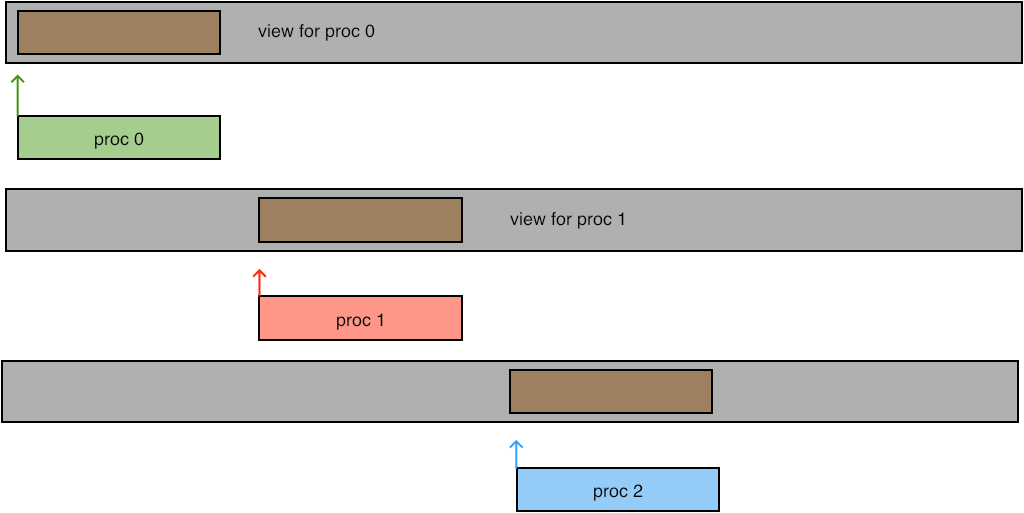
\includegraphics[scale=.4]{write-at-view}
\end{figure}

\begin{exercise}
  \label{ex:viewwrite}
  \skeleton{viewwrite}
  Write a file in the same way as in exercise~\ref{ex:blockwrite},
  but now use \indexmpishow{MPI_File_write} and use \indexmpishow{MPI_File_set_view} to set
  a view that determines where the data is written.
\end{exercise}

You can get very creative effects by setting the view to a derived
datatype.

\begin{figure}[ht]
  \label{fig:write-derived}
  \caption{Writing at a derived type}
  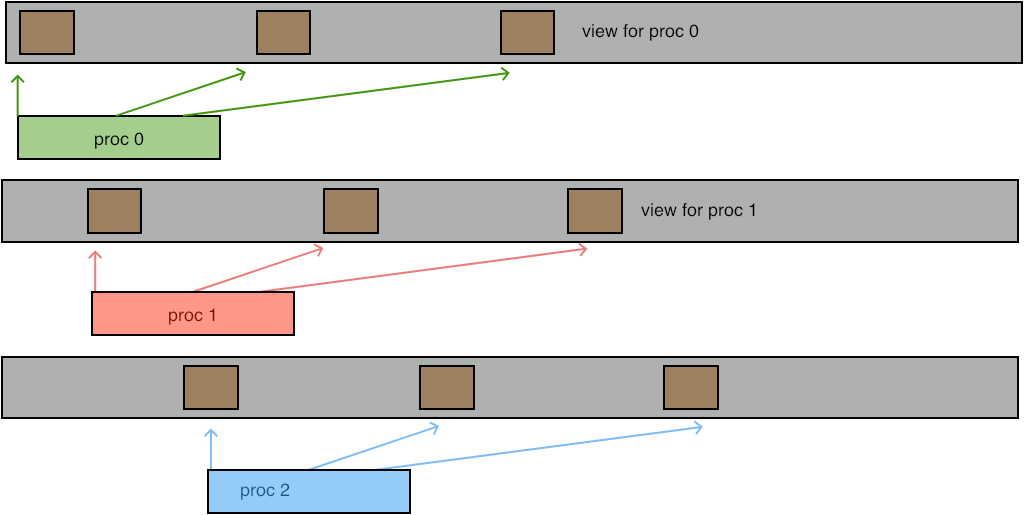
\includegraphics[scale=.4]{write-at-derived}
\end{figure}

\begin{fortrannote}{Offset literals}
  In Fortran you have to assure that the displacement parameter is of
  `kind' \indexmpishow{MPI_OFFSET_KIND}. In particular, you can not
  specify a literal zero~`0' as the displacement; use
  \indexmpidef{0_MPI_OFFSET_KIND} instead.
\end{fortrannote}

More:
\indexmpidef{MPI_File_set_size},
\indexmpidef{MPI_File_get_size}k
\indexmpidef{MPI_File_preallocate},
\indexmpidef{MPI_File_get_view}.

\Level 1 {Shared file pointers}

It is possible to have a file pointer that is shared (and therefore identical)
between all processes of the communicator that was used to open the file.
This file pointer is set with \indexmpidef{MPI_File_seek_shared}.
For reading and writing there are then two sets of routines:
\begin{itemize}
\item Individual accesses are done with \indexmpidef{MPI_File_read_shared}
  and \indexmpidef{MPI_File_write_shared}.
  Nonblocking variants are \indexmpidef{MPI_File_iread_shared}
  and \indexmpidef{MPI_File_iwrite_shared}.
\item Collective accesses are done with \indexmpidef{MPI_File_read_ordered}
  and \indexmpidef{MPI_File_write_ordered}, which execute the operations
  in order ascending by rank.
\end{itemize}

Shared file pointers require that the same view is used on all processes.
Also, these operations are less efficient because of the need to maintain the
shared pointer.

\Level 0 {Consistency}

It is possible for one process to read data previously writte by another process.
For this, it is of course necessary to impose a temporal order,
for instance by using \indexmpishow{MPI_Barrier},
or using a zero-byte send from the writing to the reading process.

However, the file also needs to be declared
\emph{atomic}\index{atomic operation!file}:
\indexmpidef{MPI_File_set_atomicity}.

\Level 0 {Constants}

\indexmpishow{MPI_SEEK_SET} used to be called \indextermtt{SEEK_SET}
which gave conflicts with the C++ library. This had to be circumvented
with
\begin{verbatim}
make CPPFLAGS="-DMPICH_IGNORE_CXX_SEEK -DMPICH_SKIP_MPICXX"
\end{verbatim}
and such.

\Level 0 {Error handling}
\label{sec:mpi-file-err}

By default, MPI uses \indexmpishow{MPI_ERRORS_ARE_FATAL} since parallel errors
are almost impossible to recover from.
File handling errors, on the other hand, are less serious:
if a file is not found, the operation can be abandoned.
For this reason, the default error handler for file operations
is \indexmpishow{MPI_ERRORS_RETURN}.

The default I/O error handler can be queried and set with
\indexmpishow{MPI_File_get_errhandler} and 
\indexmpishow{MPI_File_set_errhandler} respectively,
passing \indexmpishow{MPI_FILE_NULL} as argument.

\index{MPI/O|)}

\newpage
\Level 0 {Review questions}

\begin{tacc}
  \begin{exercise}
    T/F?
    After your \indexterm{SLURM} job ends, you can copy
    from the login node
    the files you've written to \verb+\tmp+. 
\end{exercise}
\end{tacc}

\begin{exercise}
  T/F?
  File views (\indexmpishow{MPI_File_set_view}) are intended to
  \begin{itemize}
  \item write MPI derived types to file; without them you can only write
    contiguous buffers;
  \item prevent collisions in collective writes; they are not needed for
    individual writes.
  \end{itemize}
\end{exercise}

\begin{exercise}
  The sequence \indexmpishow{MPI_File_seek_shared}, \indexmpishow{MPI_File_read_shared}
  can be replaced by \indexmpishow{MPI_File_seek}, \indexmpishow{MPI_File_read}
  if you make what changes?
\end{exercise}
